\section{Method}
\label{sec:method}

\TODO{Pipeline figure (Fig.~\ref{fig:pipeline}): camera $\rightarrow$
per-person perception $\rightarrow$ Layer 1 $\rightarrow$ Layer 2
$\rightarrow$ arbitration $\rightarrow$ Move/StopMove.}

\subsection{Per-person perception}
Colour and depth frames from an Orbbec RGB-D camera mounted on the robot
\TODO{model, resolution, fps}, with depth aligned to colour, are processed on
a laptop. A
multi-person pose model~\cite{bazarevsky2020blazepose} returns body landmarks
for up to six people, which are tracked across frames by nearest shoulder
centre. For each person $p$ at time $t$ we compute:
\begin{itemize}
\item \emph{distance} $d$, the median depth sampled on the shoulder and hip
  landmarks; its uncertainty $\sigma_d$ combines the spread of those samples,
  the fraction of invalid depth pixels and the temporal standard deviation.
  When depth is missing, $d$ falls back to apparent shoulder width with a
  larger $\sigma_d$;
\item \emph{approach speed} $v$, the smoothed negative derivative of $d$;
\item \emph{facing} $f\in[0,1]$, combining head yaw (nose position between
  the ears, weighted by eye visibility) and body yaw (shoulder depth
  difference); $\sigma_f$ grows as landmark visibility drops and as $f$
  fluctuates;
\item \emph{gaze} $g\in[0,1]$, from iris landmarks relative to the eye
  corners combined with head yaw; $\sigma_g$ grows as the inter-ocular
  distance in pixels shrinks, so gaze becomes uninformative at long range.
  \TODO{exact formula once implemented}
\end{itemize}
Hands are detected with~\cite{zhang2020mediapipehands} and assigned to the
person whose wrist landmark is nearest, normalised by shoulder width (at most
0.7 shoulder widths). Each hand is classified by an 18-class keypoint
classifier~\TODO{cite source / training data}; labels are smoothed per person
by majority vote over seven frames, and confidence $c$ is the mean softmax
probability of the winning label times its vote share.

\subsection{Layer 1: engagement}
Distance uses three sets following Hall's proxemic
zones~\cite{hall1966hidden} (NEAR, MID, FAR); facing and gaze have LOW and
HIGH; approach speed has AWAY, STILL and TOWARD. The rule base
\TODO{final rule table, e.g.\ Table~\ref{tab:rules}} maps these to
singleton engagement consequents, e.g.\ \emph{if facing is HIGH and distance
is MID then $E=0.85$}; \emph{if approach is AWAY then $E=0.10$}.

In the IT2 system every set is built as in Eq.~\eqref{eq:um-gauss} with
\begin{equation}
[m_1,m_2]=[\,m-k\,\sigma_x(p,t),\; m+k\,\sigma_x(p,t)\,],
\label{eq:fou}
\end{equation}
where $\sigma_x(p,t)$ is the measured uncertainty of input $x$ for person $p$
at frame $t$ and $k$ is a single scale factor. Rule firing uses the minimum
t-norm, and exact KM type reduction (Eq.~\eqref{eq:km}) gives
$[\Elow,\Ehigh]$. When all $\sigma_x=0$ the system is identical to the
Type-1 system with the same sets and rules, so the two differ only in the use
of measured uncertainty.

\begin{figure}[t]
\centering
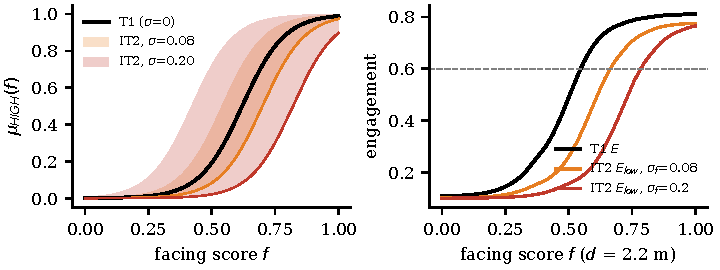
\includegraphics[width=\linewidth]{figures/fou}
\caption{Left: the facing-HIGH set for three uncertainty levels. Right:
engagement versus facing score for a person at 2.2\,m. As uncertainty grows,
the IT2 lower bound needs a clearer view before it crosses the acceptance
threshold (dashed).}
\label{fig:fou}
\end{figure}

\subsection{Layer 2: decision and arbitration}
A gesture with label $\ell$ and confidence $c$ from person $p$ is accepted if
\begin{equation}
\Elow(p,t)\ge\theta_E(\ell)\quad\wedge\quad c\ge\theta_c,
\label{eq:decision}
\end{equation}
with $\theta_E=0.60$ for motion commands, a lower $\theta_E=0.45$ for STOP
(a safety bias), and $\theta_c=0.45$. The Type-1 policy uses its crisp $E$.
A decision must persist for three frames. If several people are accepted at
once, STOP wins; otherwise the most engaged person wins. Commands are sent as
velocity set-points at 10\,Hz with a 0.3\,m/s cap, and the robot stops 0.5\,s
after the last accepted gesture. All thresholds were set on a development
recording and frozen before the test sessions.
